\section{Related Work}

\subsection{Baking Appearance onto Explicit Geometry}
Baking precomputes an object's appearance into reusable textures~\citep{RealTimeRendering}.
Deferred Neural Rendering generalized this recipe by storing learned feature textures on the mesh and decoding them in screen space~\citep{DNR}.
With the advent of NeRF~\citep{NeRFVanilla}, baking became a conversion problem:
trained fields are distilled into sparse feature grids~\citep{bakingNeRF}, textured polygon soups~\citep{MobileNeRF}, watertight meshes~\citep{bakedSDF}, or deformable avatars~\citep{bakedAvatar},
as well as differentiable inverse rendering recovers meshes, materials, and lighting directly from images~\citep{nvdiffrec},
and neural textures can be synthesized over curved surfaces~\citep{nerfTexture}.
These methods deliver genuine assets, but their view-dependent capacity is an afterthought:
low-order SH lobes or small per-pixel decoders biased toward diffuse content.
Our pipeline retains the deferred, texture-like structure of this line
while devoting explicit model capacity to sharp specularity.
In addition, methods above presuppose a global UV atlas,
whose seam-cutting and packing remain tedious to author and non-differentiable to optimize;
by anchoring appearance in per-face barycentric coordinates, our formulation sidesteps this requirement entirely. Per-face texturing such as Ptex~\citep{ptex} likewise removes the atlas, but its static per-face textures cannot represent the high-frequency, view-dependent reflection that continuous splat representations later captured.

\subsection{Modeling View-Dependent Appearance}
A parallel line of work asks how to reconstruct sharp specular transport in the first place.
Ref-NeRF reparameterizes outgoing radiance about the reflected view direction,
substantially improving specular fidelity within a volumetric field~\citep{refnerf}.
In the splatting regime, recent methods evaluate reflections in screen space against a learned environment map:
GaussianShader attaches simplified shading functions to each splat~\citep{gaussianShader},
3DGS-DR defers reflection evaluation to a per-pixel normal buffer~\citep{3dgsDR},
Ref-Gaussian incorporates physically based deferred shading~\citep{refgs},
and Spec-Gaussian replaces spherical harmonics with anisotropic spherical Gaussians~\citep{specGaussian}.

Whether it is an evaluated BRDF~\citep{cookTorrance} against a prefiltered environment map, as in classical real-time physically based shading~\citep{karis2013pbr, RealTimeRendering},
or learned as above, environment-map reflection shares one limitation: it assumes all incident light arrives from infinitely far away.
Reducing a reflection to a single directional lookup, it cannot represent near-field self-reflection or self-occlusion, the light an object casts back onto itself.
Recovering these effects generally requires tracing secondary rays~\citep{refgs, 3dgsRayTracing}, which reintroduces the very queries that rasterization avoids.
We instead handle self-reflection geometrically: because a convex part can neither occlude nor reflect itself,
we split an object into near-convex parts via convex decomposition~\citep{coacd}, each carrying its own environment map,
grown as an adaptive hierarchy that isolates high-error regions, so that self-reflection reduces to local lookups rather than recursive rays.

These methods solve specular \emph{reconstruction}, yet all of them operate on free-form primitives in ambient $\mathbb{R}^3$:
they expose no solid surface, retain the global depth sort,
and produce nothing that can be baked onto a given mesh.
Naively binding them to a fixed surface only forces them co-planar and destabilizes the sort;
our surface-bound 2D formulation sidesteps this by construction, requiring no sorting at all.
\begin{figure}[t]
    \centering
    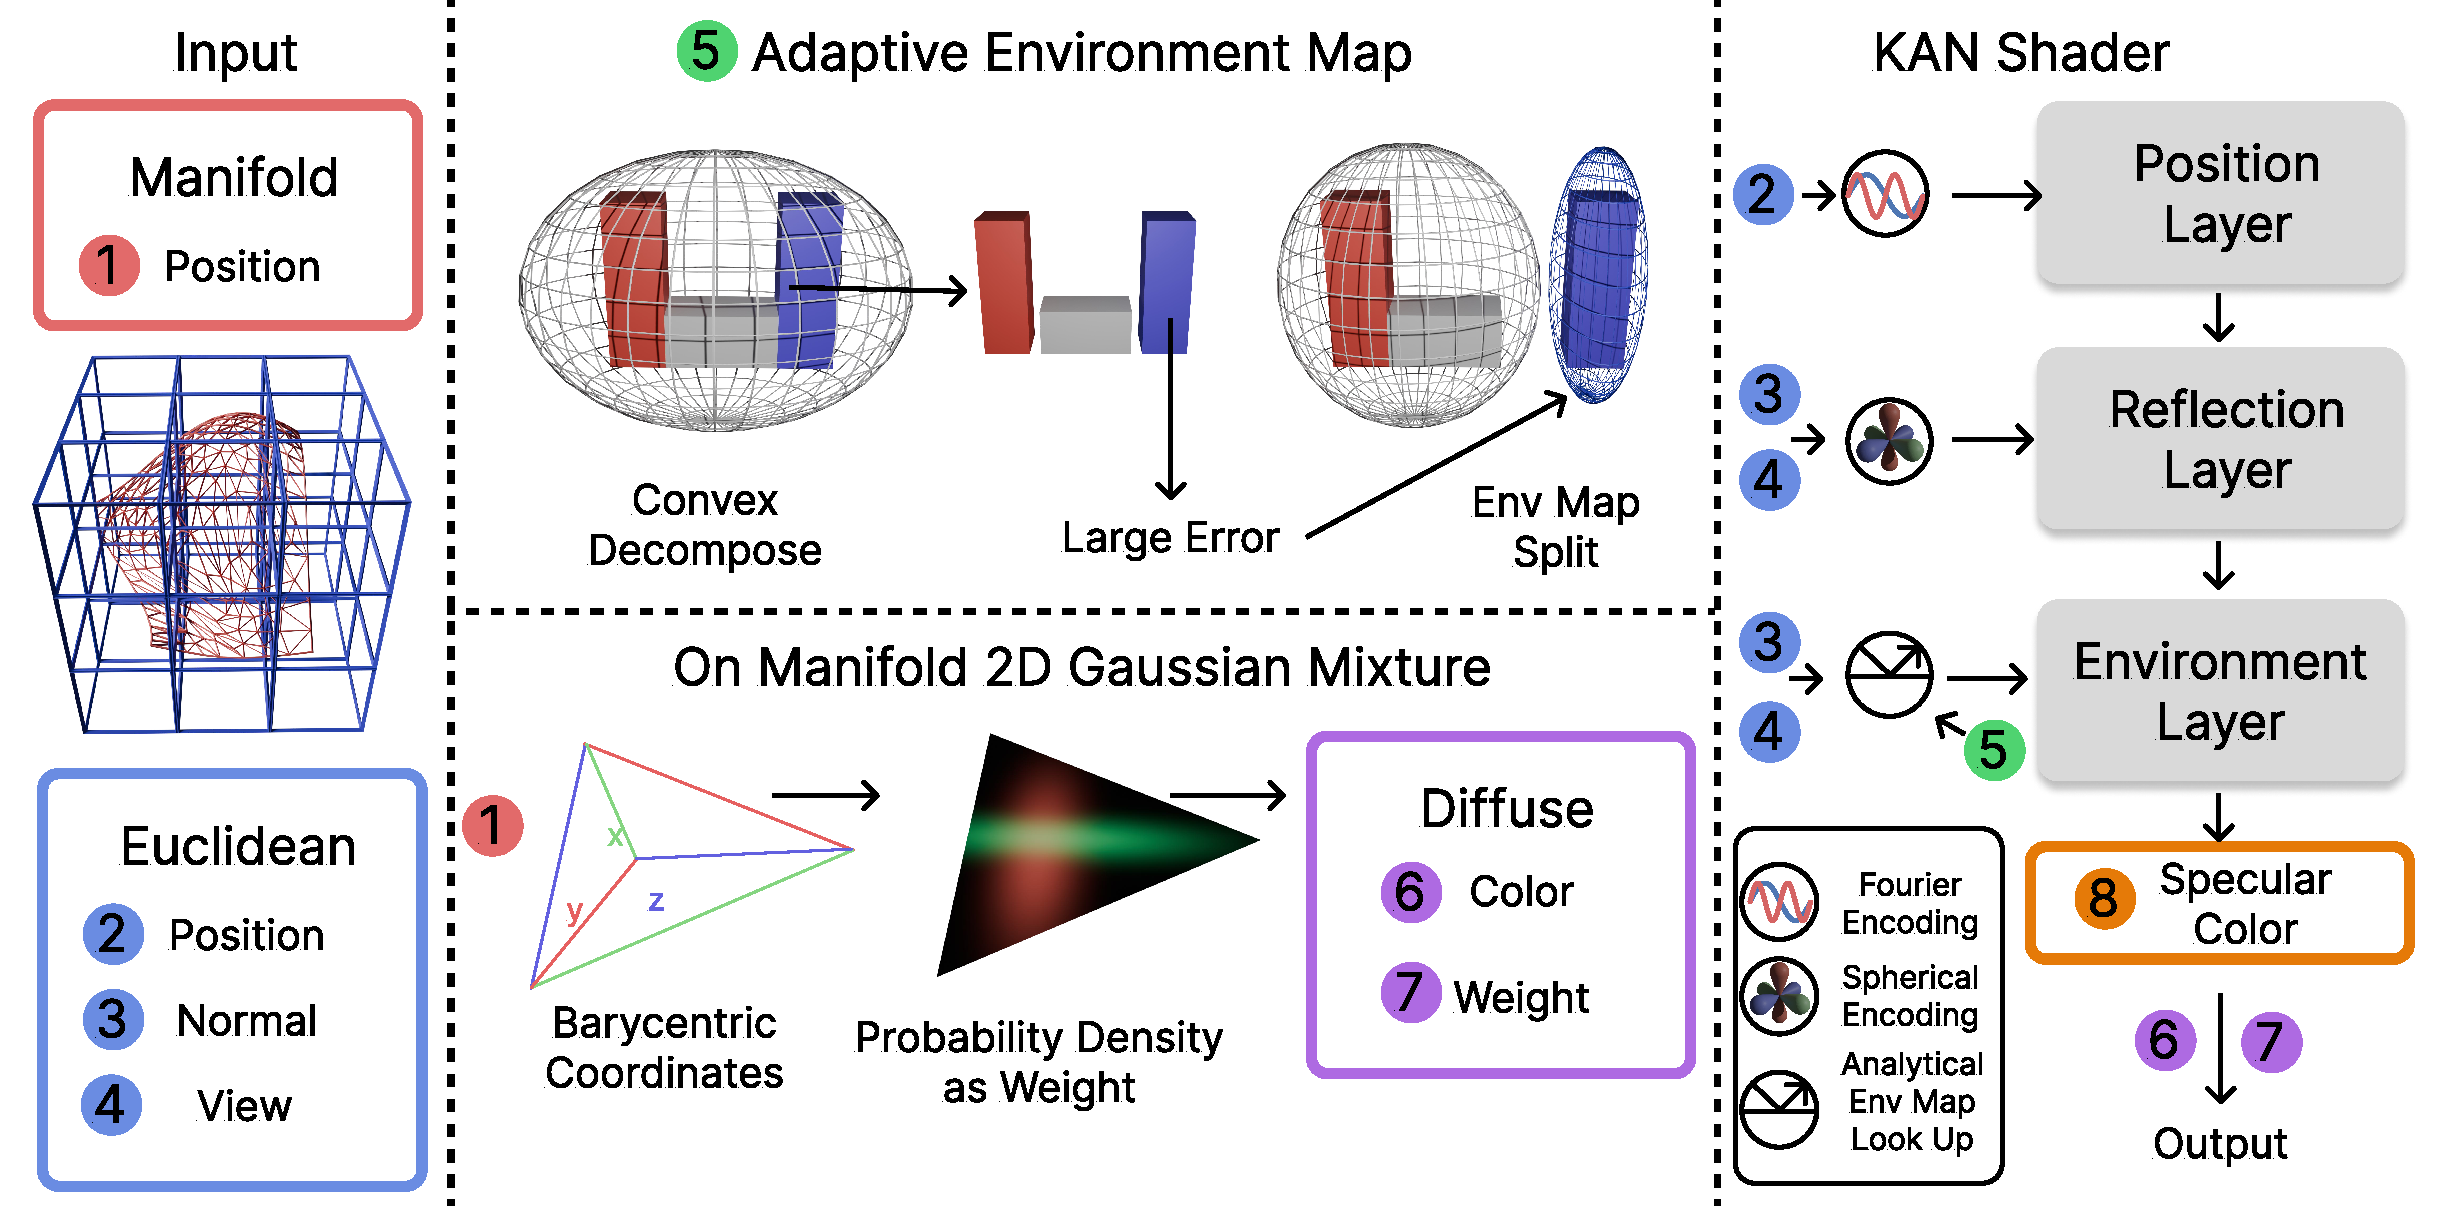
\includegraphics[width=\linewidth]{figs/method.pdf}
    \caption{%
    \textbf{Pipeline overview.}
    \emph{Input:} two position types---the on-manifold surface position \mtdone{} (barycentric coordinates on a mesh face) and the Euclidean position \mtdtwo{}, plus the surface normal \mtdthree{} and view direction \mtdfour{}.
    \emph{On-manifold 2D Gaussian mixture} (Sec.~\ref{sec:gmm}): from the barycentric position \mtdone{} we gather nearby surface Gaussians by their probability density (a partition-of-unity weight), giving the diffuse color \mtdsix{} and per-point reflectivity \mtdseven{}.
    \emph{Adaptive environment map} \mtdfive{} (Sec.~\ref{sec:env}): the object is convex-decomposed into near-convex parts, and the highest-error region is recursively split off into its own map.
    \emph{KAN shader} (Sec.~\ref{sec:kan}): a FastKAN decoder consumes the Fourier-encoded position \mtdtwo{} (Position Layer), the spherically-encoded normal \mtdthree{} and view \mtdfour{} (Reflection Layer), and an analytical lookup into the environment map \mtdfive{} (Environment Layer), producing the specular color \mtdeight{}.
    \emph{Output:} the final color composites the specular \mtdeight{} with the diffuse color \mtdsix{} gated by the reflectivity \mtdseven{}, i.e.\ Eq.~\eqref{eq:appearance}.%
    }
    \label{fig:method}
    \vspace{-4mm}
\end{figure}

\subsection{Attaching Radiance Fields to Surfaces}
A third line pushes radiance distributions toward surfaces.
Flattened kernels such as 2D Gaussian disks~\citep{2DGS} and Gaussian surfels~\citep{gaussianSurfels}
collapse one axis of the kernel to improve geometric accuracy, yet the primitives still float freely in $\mathbb{R}^3$. Mesh-scaffolded methods go further: SuGaR regularizes splats toward an extracted mesh~\citep{sugar},
GaMeS parameterizes Gaussians on triangle faces to enable editing~\citep{games},
SplattingAvatar embeds splats in a deformable template for animation~\citep{splattingAvatar},
and Texture-GS learns a UV mapping so that a 2D texture colors the splats~\citep{textureGS}.
In every case, however, the mesh merely \emph{drives} the kernels:
the rendered primitives remain three-dimensional, ambient-space objects composited by depth sorting,
and the domain of the appearance field never becomes the surface itself.
\citet{neumesh} bind learnable codes on the vertices, but never allow the code representation to float inside the 2D manifold.
The original EWA surface splatting~\citep{EWA} is, moreover, not differentiable.
In contrast, we define a strictly 2D, sort-free Gaussian mixture expressed in the barycentric coordinates on  the faces that is differentiable and free inside the 2D manifold.
In this way the mesh is not scaffolding but the domain, and it remains the authoritative solid geometry for collision, physics, and animation.


